\documentclass[bachelor,german]{hgbthesis}
% Zul�ssige Class Options: 
%   Typ der Arbeit: diplom, master (default), bachelor, praktikum 
%   Hauptsprache: german (default), english
%%------------------------------------------------------------

\graphicspath{{images/}}    % wo liegen die Bilder?
\AddBibFile{literatur.bib}  % Angabe der BibTeX-Datei

%%%----------------------------------------------------------
\begin{document}
%%%----------------------------------------------------------

% Eintr�ge f�r ALLE Arbeiten: --------------------------------
\title{Erkennung, Verfolgung und Klassifizierung von Schiffen
und Booten auf der Spree anhand des Videostreams einer IP-Kamera}
\author{Marcel Schwittlick}
\studiengang{Angewandte Informatik}
\studienort{HTW Berlin}
\abgabedatum{2013}{02}{05}	% {YYYY}{MM}{DD}

%% f�r Bachelorarbeit und Praktikumsbericht entsprechende Eintr�ge erg�nzen:

%%% zus�tzlich f�r eine Bachelorarbeit: ---------------------
\nummer{s0529494}   % XX...X = Stud-ID, z.B. 0310238045-A  
                        % (A = 1. Bachelorarbeit)
\semester{Wintersemester 2013 / 2014} 
\gegenstand{Bachelor Thesis} 
\betreuer{Prof. Dr. Frank ~Bauern�ppel, Prof. Dr. Albrecht Fortenbacher} % oder \betreuerin{..}

\strictlicense  % erzeugt restriktive Lizenzformel

%%%----------------------------------------------------------
\frontmatter
\maketitle
\tableofcontents
%%%----------------------------------------------------------

\chapter{Vorwort} 	% engl. Preface



Dies ist \textbf{Version \hgbthesisDate} der \latex-Dokumentenvorlage f�r 
verschiedene Abschlussarbeiten an der FH Hagenberg, die mittlerweile auch 
an anderen Hochschulen im In- und Ausland gerne verwendet wird.

Das Dokument entstand urspr�nglich auf Anfragen von Studierenden,
nachdem im Studienjahr 2000/01 erstmals ein offizieller
\latex-Grundkurs im Studiengang Medientechnik und -design an der
FH Hagenberg angeboten wurde. Eigentlich war die Idee, die bereits
bestehende \emph{Word}-Vorlage f�r Diplomarbeiten "`einfach"' in
\latex\ zu �bersetzen und dazu eventuell einige spezielle
Erg�nzungen einzubauen. Das erwies sich rasch als wenig
zielf�hrend, da \latex, \va was den Umgang mit Literatur und
Graphiken anbelangt, doch eine wesentlich andere Arbeitsweise
verlangt. Das Ergebnis ist -- von Grund auf neu geschrieben und
wesentlich umfangreicher als das vorherige Dokument --
letztendlich eine Anleitung f�r das Schreiben mit \latex, erg�nzt
mit einigen speziellen (mittlerweile entfernten) Hinweisen f�r \emph{Word}-Benutzer.
Technische Details zur aktuellen Version finden sich in Anhang \ref{ch:TechnischeInfos}.

W�hrend dieses Dokument anfangs ausschlie�lich f�r die Erstellung
von Diplomarbeiten gedacht war, sind nunmehr auch  
\emph{Masterarbeiten}, \emph{Bachelor\-arbeiten} und \emph{Praktikumsberichte} 
abgedeckt, wobei die Unterschiede bewusst gering gehalten wurden.

Bei der Zusammenstellung dieser Vorlage wurde versucht, mit der
Basisfunktionalit�t von \latex das Auslangen zu finden und -- soweit m�glich --
auf zus�tzliche Pakete zu verzichten. Das ist nur zum Teil gelungen;
tat\-s�ch\-lich ist eine Reihe von erg�nzenden "`Paketen"' notwendig, wobei jedoch
nur auf g�ngige Erweiterungen zur�ckgegriffen wurde.
Selbstverst�ndlich gibt es dar�ber hinaus eine Vielzahl weiterer Pakete,
die f�r weitere Verbesserungen und Finessen n�tzlich sein k�nnen. Damit kann
sich aber jeder selbst besch�ftigen, sobald das notwendige Selbstvertrauen und
gen�gend Zeit zum Experimentieren vorhanden sind.
Eine Vielzahl von Details und Tricks sind zwar in diesem Dokument nicht explizit
angef�hrt, k�nnen aber im zugeh�rigen Quelltext jederzeit ausgeforscht
werden.

Zahlreiche KollegInnen haben durch sorgf�ltiges Korrekturlesen und
konstruktive Verbesserungsvorschl�ge wertvolle Unterst�tzung
geliefert. Speziell bedanken m�chte ich mich bei Heinz Dobler f�r
die konsequente Verbesserung meines "`Computer Slangs"', bei
Elisabeth Mitterbauer f�r das bew�hrte orthographische Auge und
bei Wolfgang Hochleitner f�r die Tests unter Mac~OS.

Die Verwendung dieser Vorlage ist jedermann freigestellt und an
keinerlei Erw�hnung gebunden. Allerdings -- wer sie als Grundlage
seiner eigenen Arbeit verwenden m�chte, sollte nicht einfach
("`ung'schaut"') darauf los werken, sondern zumindest die
wichtigsten Teile des Dokuments \emph{lesen} und nach M�glichkeit
auch beherzigen. Die Erfahrung zeigt, dass dies die Qualit�t der
Ergebnisse deutlich zu steigern vermag.


Der Quelltext zu diesem Dokument sowie das zugeh�rige
\latex-Paket sind in der jeweils aktuellen Version online
verf�gbar unter
%
\begin{quote}
\url{www.fh-hagenberg.at/staff/burger/diplomarbeit/}
%\href{www.fh-hagenberg.at/staff/burger/diplomarbeit/}{www.fh-hagenberg.at/staff/burger/diplomarbeit/}
\end{quote}
%
oder auch unter
%
\begin{quote}
\url{http://elearning.fh-hagenberg.at/} \newline
im Kurs "`Anleitung/Vorlage f�r Master-/Bachelor-/Diplomarbeiten"'.
%\url{http://theses.fh-hagenberg.at}
\end{quote}
%
Trotz gro�er M�he enth�lt dieses Dokument zweifellos Fehler und Unzul�nglichkeiten
-- Kommentare, Verbesserungsvorschl�ge und passende Erg�nzungen
sind daher stets willkommen, am einfachsten per E-Mail direkt an mich:
\begin{center}%
\begin{tabular}{l}
\nolinkurl{wilhelm.burger@fh-hagenberg.at} \\
Dr.\ Wilhelm Burger \\
FH Hagenberg -- Digitale Medien\\
Austria
\end{tabular}
\end{center}

\noindent
�brigens, hier im Vorwort (das bei Diplomarbeiten �blich, bei Bachelorarbeiten 
aber entbehrlich ist) kann man kurz auf die Entstehung  des Dokuments eingehen.
Hier ist auch der Platz f�r allf�llige Danksagungen (\zB an den Betreuer, 
den Begutachter, die Familie, den Hund, ...), Widmungen und philosophische 
Anmerkungen. Das sollte man allerdings auch nicht �bertreiben und sich auf 
einen Umfang von maximal zwei Seiten beschr�nken.




		% ggfs. weglassen
\chapter{Kurzfassung}
Diese Bachelorarbeit besch�ftigt sich mit der Aufgabenstellung anhand eines Bildsequenz Objekte zu erkennen und zu verfolgen. Diese Bildsequenz soll anhand einer IP-Kamera aufgezeichnet werden, damit sie �ber das Internet von jedem Ort der Welt ausgewertet werden kann.
Bei den Objekten, die zu erkennen und verfolgen sind handelt es sich um Schiffe und Boote auf einem Fluss. 

Zus�tzlich soll untersucht werden, ob und wenn ja, inwiefern die erkannten Objekte klassifiziert werden k�nnen, um gegebenenfalls Muster im Schiffsverkehr erkennen zu k�nnen. M�gliche Anhaltspunkte f�r Klassifikatoren k�nnen Eigenschaften der Schiffe, wie Typ, Gr��e, und Geschwindigkeit sein.

Der praktische Teil dieser Arbeit soll aus einem Prototypen bestehen, welche den gefunden L�sungsansatz demonstriert. Dieser Prototyp soll aus einer Hardware- und einer Softwarekomponente bestehen.

Die Erkennung, Verfolgung und Klassifizierung soll mittels bekannter und bereits implementierter Computer Vision Algorithmen geschehen und es soll untersucht werden, inwiefern das System m�glichst robust gegen�ber Wettereinfl�ssen erstellt werden kann. Es soll ein theoretischer Ansatz zur Klassifikation der Schiffe entwickelt werden, welche nicht teil der praktischen Arbeit sein soll.
\chapter{Abstract}
The main goal of the Bachelor thesis is to detect and track ships and boats on a live video stream. Further it is to research by which properties the boats can be classified, in order to 
create some sort of patterns and statistics about the traffic on the river. 
The hardware of the system needs to be developed, in order to create a weatherproff installation of the camera. The prototype is supposed to be portable to any other part of the river, whereas the system needs to be adjustablable to other environments, like different lighting, weather and viewpoint situations. 
The detection and recognition of the boats is going to be implemented using known and common computer vision algorithms and is supposed to be resistent to different weather infliences. For classifying the boats, methods of machine learning are supposed to be researched and compared to other approaches.

%%%----------------------------------------------------------
\mainmatter         % Hauptteil (ab hier arab. Seitenzahlen)
%%%----------------------------------------------------------

\chapter{Einleitung}
In den folgenden Kapiteln wird beschrieben, wiö das Problem dieser Bachelor Arbeit angegangen wurde.

\begin{enumerate}
\item \textbf{Einführung }: Was ist die Problem- oder Aufgabenstellung und warum sollte man sich dafür interessieren?
\item \textbf{Analyse / Präzisierung des Themas}:Zunächst wird die Aufgabe näher analysiert. Hier beschreibt man den aktuellen Stand der Technik oder Wissenschaft ("`State-Of-The-Art"'), zeigt bestehende
							Defizite oder offene Fragen auf und entwickelt daraus die Sto\ss{}richtung der eigenen Arbeit.
\item \textbf{Definition}:Daraus ergibt sich eine Definition des Problemes und der naechsten Handlungsschritte.
\item \textbf{Grundlagen}:Dann werden die Grundlagen der Definierten Ziele beschrieben.
\item \textbf{Entwurf / Eigener Ansatz}:Anschliessend wird ein Entwurf des zu entwickelnden Systemes dargelegt.
\item \textbf{Implementierung / Prototyp}:Woraus eine tatsaechliche Implementierung resuliert.
\item \textbf{Test}:Welche getestet werden muss.
\item \textbf{Fazit / Zusammenfassung}:Und durch ein Fazit abgerundet wird.
\end{enumerate}

\section{Motivation}
Für die Entwicklung solche eines Systemes gibts es für den Autor dieser Arbeit diverse Motivationen. Das wichtigste Motiv ist es dem Autor eine Möglichkeit zu geben sich umfangreich und selbstständig mit dem Thema der Computer Vision zu beschäftigen. Die Thematik Informationen über Objekte und deren Zusammenhang anhand von Bildern und Bildersequenzen zu gelangen faszinierte den Autor bereits seit einiger Zeit. Weiterhin hatte der Autor noch nie die Gelegenheit sich mit der Thematik des Maschinellen Lernens auseinanderzusetzen, wo diese Arbeit das Potenzial bietet gro\ss{}en gebrauch davon zu machen.
Im Zusammenhang damit steht, dass der Autor von den Neuigkeiten und Nachrichten bezüglich der \"Uberwachungssysteme im In- und Ausland verwirrt ist und mit eigenen Fähigkeiten herausfinden möchte, inwiefern diese \"Uberwachungssysteme tatsächlich funktionieren und wozu sie in der Lage sind. In den Nachrichten wurde in den letzten Jahren verhäuft über Städte(London) und Situationen(Terroranschlag Boston) berichtet. Dazu möchte der Autor herausfinden, wozu solche Systeme technisch in der Lage sind, und was für einen potenziellen Gewinn an Sicherheit sie versprechen können.

\"Uber diese persönliche Motivation hinaus bietet die Entwicklung eines solchen Systemes gro\ss{}en \"Okonomischen Wert, da dadurch Statistiken und Informationen über den Schiffsverkehr an unterschiedlichen Stellen des gleichen Flusses verglichen werden können, um daraus Schlüsse über ??? zu ziehen.

\section{Relevanz}
\section{Aufbau der Arbeit}
\chapter{Anforderungsanalyse}
In der Bachelorarbeit soll es darum gehen Schiffe bzw. Boote anhand eines Live-Videostreames zu erkennen und zu tracken. Zus�tzlich soll untersucht werden, inwiefern die Schiffe nach bestimmten
Kriterien klassifiziert werden k�nnen, um gegebenenfalls Muster im Flussverkehr erkennen zu
k�nnen. M�gliche Klassifikatoren k�nnen der Schifftyp, die Gr��e des Schiffes und die
Geschwindigkeit des Schiffes sein. Dadurch k�nnen detaillierte Statistiken �ber einen bestimmten
Flussabschnitt erstellt werden, welche gegebenenfalls mit Statistiken anderer Flussabschnitte
verglichen werden k�nnen. 
Deswegen soll die Hardwarekomponente des Systemes portabel und
resistent gegen�ber Wettereinfl�ssen sein. Die Entwicklung der Hardware Komponente soll
ebenfalls Teil der Arbeit sein und aus einer IP-Kamera inklusive Wetterresistenter Halterung
bestehen. Es soll ein funktionierender Prototyp erarbeitet werden, der mit wenigen Schritten an
einen anderen Ort umgezogen werden kann. Dies erfordert h�chstwarscheinlich eine Art
Kalibrierung des Systemes auf die ver�nderten Umgebungsfaktoren, wie Blickwinkel und
Lichtverh�ltnisse des neuen Ortes, welche elementarer Teil des Systemes sein soll.
Die Erkennung, Verfolgung und Klassifizierung soll mittels bekannter und bereits implementierter
Computer Vision Algorithmen geschehen und m�glichst robust gegen�ber eventuellen
Wettereinfl�ssen sein. Zur Klassifizierung der Schiffe soll die Methode des Maschinellen Lernens in
Betracht gezogen werden, allerdings mit anderen Ans�tzen zur Klassifizierung verglichen werden.
Es soll eine Software entwickelt werden, welche es erm�glicht Schiffe anhand von digitalem Videosignal zu erkennen, zu verfolgen und zu klassifizieren. Dieses Problem ist ein Klassisches Problem der Computer Vision und mit den n�tigen Methoden und Mitteln umzusetzen. Allerdings soll die Software weiterhin f�r die M�glichkeit die Kamera an verschieden Orte zu stellen gestaltet werden. Durch die unterschiedlichen Positionen der Kamera muss die Software variablen gebaut sein, sodass man das System an die ge�nderten Umst�nde anpassen kann. Weiterhin muss bedacht werden, dass das Software system zu jeder Zeit w�hrend des Tages funktionieren soll und muss sich deswegen an �ndernde Wetterumst�nde anpassen k�nnen, oder so robust gebaut sein, dass sie zu jeder Jahreszeit funktioniert.

\section{Anwendungsgebiet}
Die Arbeit besch�ftigt sich mit der Thematik anhand von Bildern und Bildsequenzen ( Videos ) aussagekr�ftige Informationen zu erhalten. Ein Bild repr�sentiert im Computer speicher ist nichts weiter, als eine
Matrix mit bestimmter H�he und Breite, welche multipliziert die Pixelanzahl des Bildes angeben. An jeder Position dieser Matrix sind die Farbwerte zu dem entsprechendem Pixel gespeichert. Durch die Betrachtung dieser Pixelmatrix kann unser menschliches Gehirn ohne weiteres dem Bild Informationen �ber dessen Inhalt entnehmen, folglich das Bild zu interpretieren. Die Interpretation eines Bildes ist ein komplexes Konstrukt und ist durch unsere Erfahrung als Mensch m�glich. Mehr zu diesem Thema in einem abgesonderten Block.
Ein Computer hat allerdings kein komplexes Gehirn und sieht ein Bild, was f�r einen Menschen z.B. gro�en emotionalen Wert haben kann schlichtweg als einen zweidimensionalen Array, welcher konkrete farbwerte enth�lt.
Anhand dieser repr�sentation des Bildes kann allerdings der Computer instruiert werden bestimmte Muster zu erkennen, oder bestimmte Operationen auf das Bild anzuwenden, wodurch letztendlich dem Bild Informationen 
entnommen werden kann. Diese Verarbeitung wird maschinelles Sehen oder Bildverstehen engl. Computer Vision genannt und besch�ftigt sich damit computergest�tzt Bilder auf eine menschliche Art und Weise zu interpretieren. Das Thema maschinelles Sehen wird im Abschnitt Maschinelles Sehen n�her beschrieben.

\section{Umsetzung}
\section{Anforderungen an den Prototypen}
Der Prototyp soll in der Lage sein unter m�glichst allen Wetterumst�nden Schiffe anhand des Videostreames der IP-Kamera zu erkennen. Dies soll nur tags�ber passieren.
Dieser Prototyp soll an unterschiedlichen Orten eingesetzt werden k�nnen, gegebenenfalls soll die Kamera an einen anderen Flussabschnitt bewegt werden k�nnen und die Software soll an die dort gegebenen lokalen Umst�nde anpassbar sein. Diese Anpassung soll anhand einer Grafischen Benutzeroberfl�che geschehen.
\subsection{Hardware}
Die Hardwarekomponente des Prototypen soll aus einer Kamera bestehen, die entweder Videosinal �ber das Netzwerk / Internet an den verarbeitenden Rechner inkl. Software sendet, oder direkt an einem Computer angeschlossen sein, welcher die Verarbeitung dann direkt vor Ort vornimmt. Allerdings ergibt sich dadurch das Problem, dass ein Computer am FLuss stehen mnuss, was nicht immer m�glich ist, da eine Stromzufuhr nicht immer gegeben sein kann. ( Wie soll denn �berhaupt eine Kamera dort funktionieren? Eventuell eine Kamera per Batterie laufen lassen mit Mobilem Hotspot?!! ) 

\subsubsection{Kamera}
An die Kamera, die die Aufgabe hat den Flussausschnitt zu filmen werden nur wenige Anforderungen gestellt. Sie soll ausschlie�lich die F�higkeit haben ihren Videostream �ber das Internet erreichbar zu machen. Die Qualit�t des Videostreames ist ein Kriterium, das ausser Acht gelassen werden soll.
Als Kamera wurde die AXIS M1031-M gew�hlt, da sie schlichtweg gegeben war und den Anforderungen entspricht. Sie bietet ihren Stream in diversen Formaten ( h.264, Motion JPEG, MPEG-4 ) an und war bereits eingerichtet.
Ausserdem hat diese Kamera den Vorteil einer einfachen Installation, einer 640x480 Pixel Aufl�sung mit einer Bildrate von 30FPS.

\begin{figure}
\centering
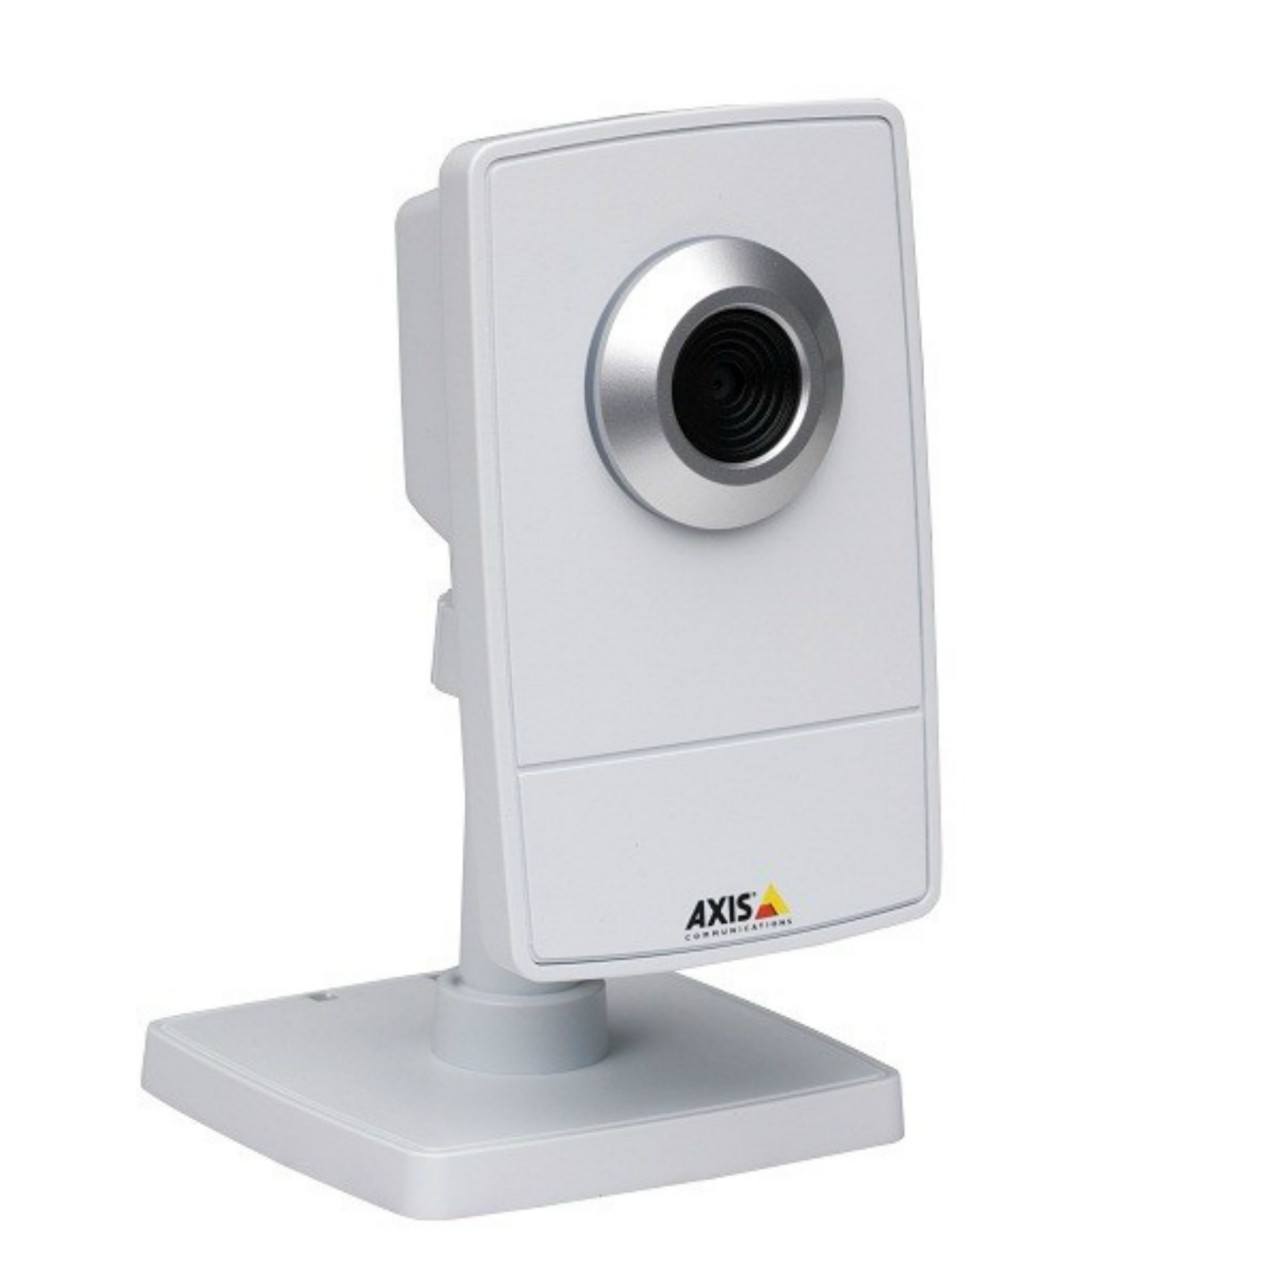
\includegraphics[width=.95\textwidth]{axis_camera} %{CS0031}
\caption[AXIS M1031-M]{AXIS M1031-M\footnotemark}
\label{fig:AXIS M1031-M}
\end{figure}
\subsubsection{Halterung}
\subsubsection{Benutzte Hardware}
\subsection{Software}
\footnotetext{\url{http://www.networkcamerastore.com/axis-m1031-w-0300-004-wireless-network-camera}}
Die Softwarekomponente des Systemes soll inder Lage sein aus einer erh�hren Position am Flussrand Schiffe zu erkennen, zu verfolgen und gegebenenfalls klassifizieren und sonstige Informationen �ber das Schiff, wie z.B. Geschwindigkeit, L�nge aufzuzeichnen. Die Position aus der die Kamera auf den Fluss 'sieht' soll variabel sein und die Sofware soll an diese ver�nderbaren Umst�nde angepasst werden k�nnen. Diese Anpassung soll anhand einer grafischen Benutzeroberfl�che geschehen k�nnen.
\subsubsection{Benutzeroberfl�che}
Die grafische Benutzeroberfl�che soll es dem Benutzer erm�glichen die Algorithmen, die zur Erkennung und Verfolgung der Schiffe bnuetzt werden fein zu parametrisieren. Dazu sollen alle entscheidenden Parameter der Algorithmen aoffen gelegt werden und durch Standard Oberfk�chen-Elemente ver�nderbar sein.
\subsubsection{Performance}
Da die Verarbeitung des Videostreames in Echtzeit geschehen soll die Software alle m�glichen Parallelisierungsmethoden benutzen, die sich anbieten. 
\section{Abgrenzungskriterien}
In diesem Abschnitt wird erl�utert von welchen Anforderungen sich der Prototyp klar abgrenzt. Dar�ber sollte ich mir mal gedanken machen-
\section{Methodik}
In den folgenden Unterabschnitten wird tiefer auf die Umsetzung des Prototypen und dieser Dokumentation eingegangen. Es werden Hilfsmittel, die das Projektmanagement und die Programmierung unterst�tzen gegeneinander abgewogen und untersucht.
\subsection{Projektmanagement}
Um ein professionelles und strukturiertes Projektmanagement zu gew�hrleisten muss ich f�r eine Unterst�tzung entschieden werden. G�ngige M�glichkeiten bieten Projektmanagement-Systeme wie trac und Redmine.
\begin{figure}
\centering
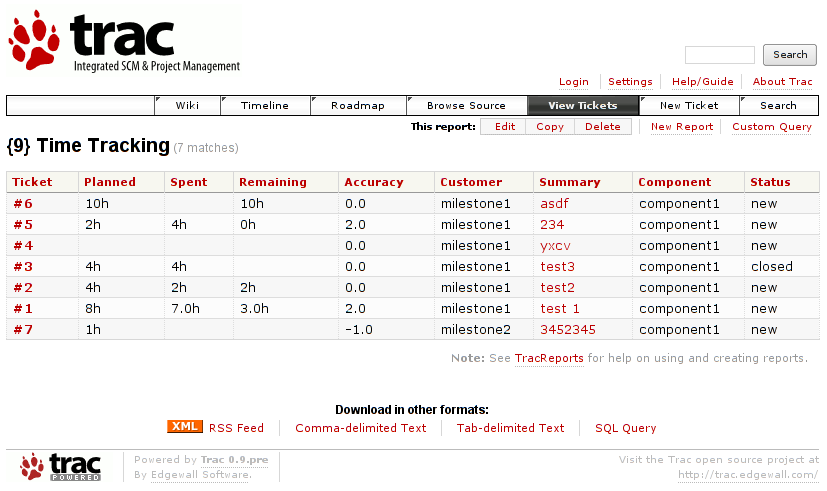
\includegraphics[width=.95\textwidth]{trac-timetracking-report} %{CS0031}
\caption[trac Projektmanagement]{trac Projektmanagement\footnotemark}
\label{fig:trac Projektmanagement}
\end{figure}
\subsection{Programmiermethodik}
\footnotetext{\url{http://trac.edgewall.org/wiki/TimeTracking}}
Bei diesem Projekt kann kein nicht-iteratives Vorgehensmodell, wie das Wasserfallmodell benutzt werden, da sich die tats�chlichen Anforderungen an die Software erst w�hrend der Implementierungsphase herausstellen. Man kann bei solch einem Projekt vorab schlichtweg nicht sagen, welche Bildverarbeitungsmethoden genau angewandt werden sollen, da nach der Implementierung zun�chst eine fundierte Untersuchung der Ergebnisse geschehen muss, um zu entscheiden, welche Folgeverarbeitungen darauf aufbauen k�nnen. Es gibt diverse Ans�tze, die das Problem dieser Arbeit l�sen, welche jedoch nicht vor tats�chlicher Implementierung festgehalten werden k�nnen.
Daher wurde sich entschieden eine agile Vorgehensweise zu w�hlen, um genau diese Art des Projektes zu addressieren. Dadurch kann sich unmittelbar an Erkenntnisse der Implementierung angepasst werden.
\subsubsection{Agile Programmierung}
\subsubsection{Extreme Programming}

\chapter{Grundlagen}
\section{Allgemein}
Der typische grundlegend strukturellen Schritte bei der Erkennung der Schiffe ist wie folgt:
Im folgenden werden s�mtliche grundlegenden Konzepte die zum Verst�ndnis der in den folgenden Kapiteln erarbeiteten L�sungsans�tze helfen erl�utert. 

Die Aufgabe Objekte anhand von Bild/-sequenzen zu erkennen und diesen Informationen �ber der realen Objekte zu entnehmen gliedert sich in die Thematik des Bildverstehens ein. Das Forschungsgebiet des Bildverstehens besch�ftigt sich damit die menschliche Art zu sehen auf eine Maschine zu �bertragen. Die visuelle Interpretation von dem was unsere Augen wahrnehmen geschieht ununterbrochen und meist unterbewusst. \cite[S.~33]{Sester95}Die Tatsache, dass der Mensch auf seine Erfahrung dar�ber, wie die Welt aufgebaut ist immer zugreifen kann erm�glicht ihm Gegenst�nde zu erkennen, die nicht ausschlie�lich dadurch, was man davon sieht gedeutet werden k�nnen, sondern aus einer Kombination von zus�tzlichen Informationen. Diese weiteren Informationen k�nnen aus anderen menschlichen Sinnen gewonnen werden, welche bei der maschinellen Bildinterpretation nicht gegeben sind. (vgl. Sester95)
\begin{quote}
Menschliches Sehen bezeichnet nach Boden den Prozess, der Bilder der realen Welt in eine f�r den Betrachter g�nstige Beschreibung �berf�hrt, bei dem nur noch die wichtigen Informationen erhalten bleiben und unwichtige entfallen.
\footnote{\url{http://www.ifp.uni-stuttgart.de/publications/dissertationen/moni_diss.pdf}}
\end{quote}
Der menschliche Sehapparat hat sich �ber den Verlauf der Evolution so entwickelt, dass er ebenfalls Objekte, die in verschiedenen Erscheinungsarten auftreten k�nnen erkennen zu k�nnen. Objekte k�nnen in unterschiedlichen Situationen 'gesehen' werden, wobei diverse Faktoren, der die �u�ere Erscheinung ver�ndern k�nnen greifen. Diese sind Faktoren wie Beleuchtung, Perspektive, Orientierung und andere Einfl�sse ein Objekt gar physisch ver�ndern. Trotzdem k�nnen diese Objekte von dem menschlichen Sehapparat erkannt werden, was grunds�tzlich damit zusammen h�ngt, dass der Mensch die F�higkeit zu lernen hat. Dadurch ist es den Menschen m�glich ununterbrochen Informationen �ber ihre Umgebung zu verarbeiten und daraus die menschliche Bildverstehen zu verbessern, um in der Zukunft visuelle Einfl�sse noch schneller und genauer zu verarbeiten und zu interpretieren.
\begin{figure}
\centering
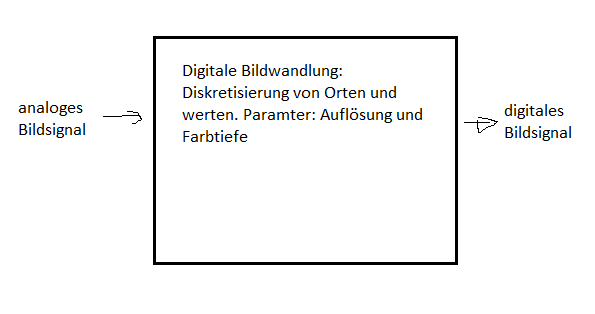
\includegraphics[width=.95\textwidth]{digitale_bildwandlung} %{CS0031}
\caption[Digitale Bildwandlung]{Digitale Bildwandlung\footnotemark}
\label{fig:Digitale Bildwandlung}
\end{figure}
\footnotetext{\url{http://people.f4.htw-berlin.de/~barthel/veranstaltungen/GLDM/GLDM.htm}}

Die allgemeine Abfolge von Schritten, die zur L�sung des Problemes dieser Arbeit f�hrt ist im folgenden dargestellt.
\begin{itemize}
\item{Szene}
\item{Bildaufnahme}
\item{Bildvorverarbeitung}
\item{Segmentierung}
\item{Merkmalsextraktion}
\item{Klassifizierung}
\item{Aussage}
\end{itemize}

\subsection{Bildverarbeitung}
%http://de.wikipedia.org/wiki/Bildverarbeitung 
%http://people.f4.htw-berlin.de/~barthel/veranstaltungen/GLDM/GLDM.htm 
Die Bildverarbeitung allgemein, allerdings im besonderen Verfahren der digitalen Bildverarbeitung erfordern Bilddaten als Eingabedaten. Als Eingabebilddaten ist die Rastergrafik am meisten verbreitet, welche ein Bild durch ein zweidimensionales Raster dargestellt wird. Eine andere Art der Bilddaten sind die Vektorgrafiken, die nicht aus Pixeln bestehen, sondern aus geometrischen Anweisungen, die das Bild aus Grafikprimitiven und geometrischen Kurven formt.

Die Bildverarbeitung liefert die entsprechenden mathematischen Verfahren, die bei der Bildbearbeitung bzw. der professionellen Ver�nderung / Analyse von digitalen Bildern zum Einsatz kommen. Die Bildveratbeitung dient als Grundlage zur Bildanalyse, Bildauswertung, Bildlkassifikation, Bilderkennung und Bildsortierung.

Der digitalen Bildverarbeitung liegen digitale Bilddaten zu grunde, die zun�chst geschaffen werden m�ssen. Dies geschieht allgemein beschrieben indem man entweder von einer Szene mit einer Digitalkamera ein Bild macht, oder ein analoges Bild scannt. Wissenschaftlich beschrieben ist eine Digitalkamera ein digitaler Bildwandler, der dazu in der Lage ist ein analoges Bildsignal abzutasten und in diskrete Werte zu �berf�hren. Diese �berf�hrung wird anhand von zwei Parametern durchgef�hrt: Aufl�sung und Farbtiefe.
Die Aufl�sung beschreibt, mithilfe von wievielen Bildpunkten eine Szene abgetastet wird, wie genau detailliert das Bild also aufgenommen wird. Die Farbtiefe beschreibt, mit wievielen Farbkan�len erzeugt wird, welche Farben f�r die Zusammenstellung des Bildes zugelassen werden und wie genau diese gespeichert werden. 

S�mtliche Bildoperatoren arbeiten auf den Daten ( Pixeln ) eines Ursprungsbildes und erzeugen daraus ein Ergebnisbild. Sie k�nnen als mathematische Bildoperation gesehen werden und k�nnen in einige Untergruppen kategorisiert werden, welche im folgenden individuell betrachtet werden.

\subsubsection{Punkoperatoren}
Bildpunktoperatoren arbeiten ausschlie�lich auf dem Farbwert(en) eines Bildpunktes des Ursprungsbildes. Sie haben als Eingabedaten die Farbwerte eines Bildpunktes und errechen ausschlie�lich die Farbwerte des Ergebnisbildes des Pixels an der gleichen Position im Bild, wie des Ursprungsbildes.
\begin{quote}
\textit{ErgebnisPixel( x, y ) = Bildpunktoperator( Ursprungsbild( x, y ) )}
\end{quote}

\begin{figure}
\centering
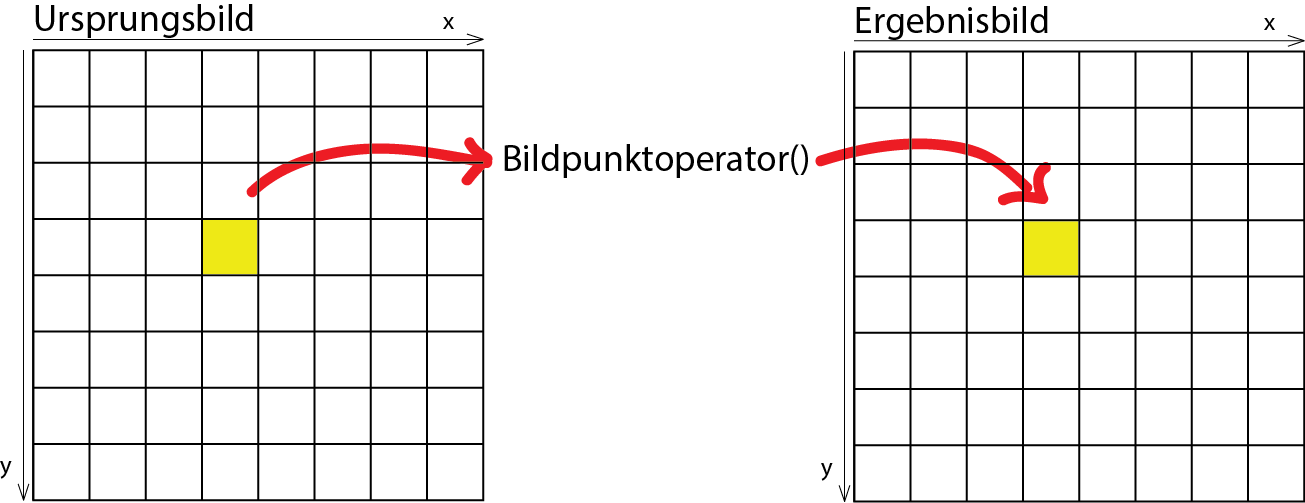
\includegraphics[width=.95\textwidth]{bildpunktoperator} %{CS0031}
\caption[Arbeitsweise von Bildpunktoperatoren]{Arbeitsweise von Bildpunktoperatoren}
\label{fig:Arbeitsweise von Bildpunktoperatoren}
\end{figure}

Mithilfe von Bildpunktoperatoren k�nnen Verarbeitungen, wie zum Beispiel Helligkeits- und Kontrastanpassungen, sowie Farbkorrekturen und Tonwertkorrekturen, aber auch Bild�berlagerungen erreicht werden.
\emph{homogen}
\emph{inhomogen}

\subsubsection{Nachbarschaftsoperatoren}
Nachbarschaftsoperatoren arbeiten als Eingabedaten auf mehreren Bildpunkten. Sie haben einen Kernel, welcher bestimmt, welche Bildpunkte um den aktiven Bildpunkt in die Berechnung des Filters mit einbezogen werden sollen. Mit Hilfe von Nachbarschaftsoperatoren k�nnen diverse Ziele, wie die Gl�ttung eines Bildes, oder Verringerung des Rauschen in Bildern, oder die Bestimmung von Kanten eines Bildes erreicht werden. Im Folgenden werden Nachbarschaftsoperatoren \emph{Filter} genannt.

\begin{quote}
\textit{ErgebnisPixel( x, y ) = Operator( KernelUrsprungsbild( x, y ) )}
\end{quote}

\begin{figure}
\centering
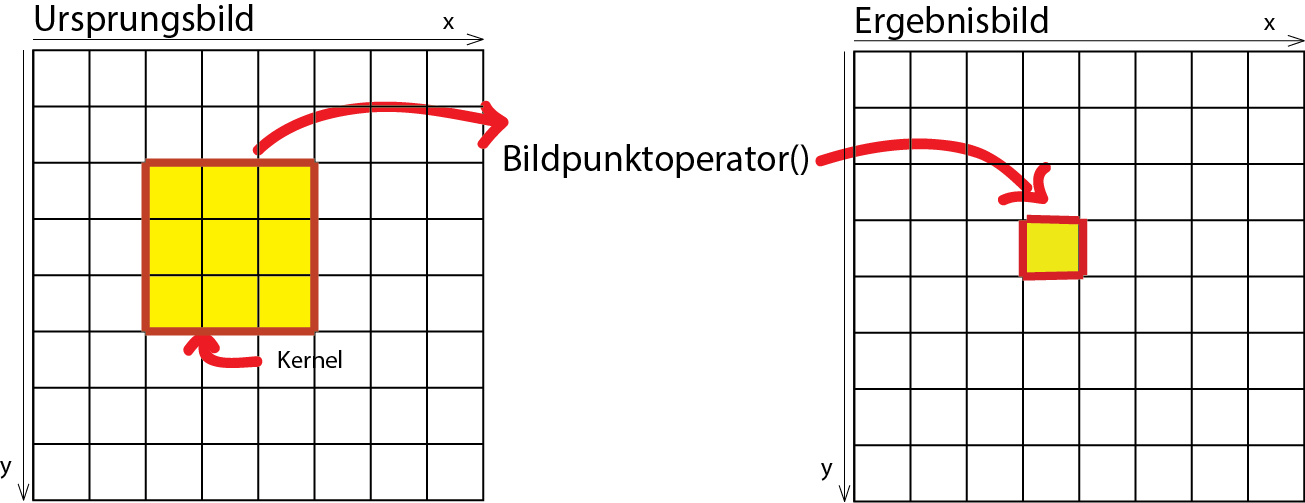
\includegraphics[width=.95\textwidth]{nachbarschaftsoperator} %{CS0031}
\caption[Arbeitsweise von Nachbarschaftsoperatoren]{Arbeitsweise von Nachbarschaftsoperatoren}
\label{fig:Arbeitsweise von Nachbarschaftsoperatoren}
\end{figure}

\emph{Faltungsfilter}
\emph{Medianfilter}
Der Medianfilter ist ein Filter, der zur Reduktion von Bildrauschen dient.
\begin{figure}
\centering
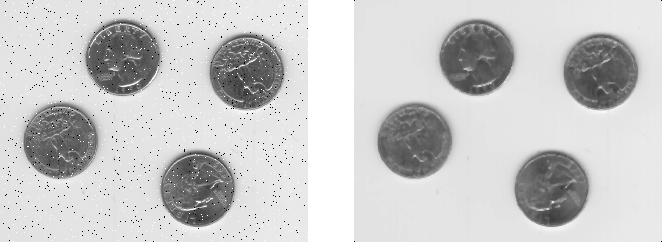
\includegraphics[width=.95\textwidth]{saltnpepper_median_coins} %{CS0031}
\caption[Medianfilter]{Medianfilter\footnotemark}
\label{fig:Medianfilter}
\end{figure}
\begin{figure}
\centering
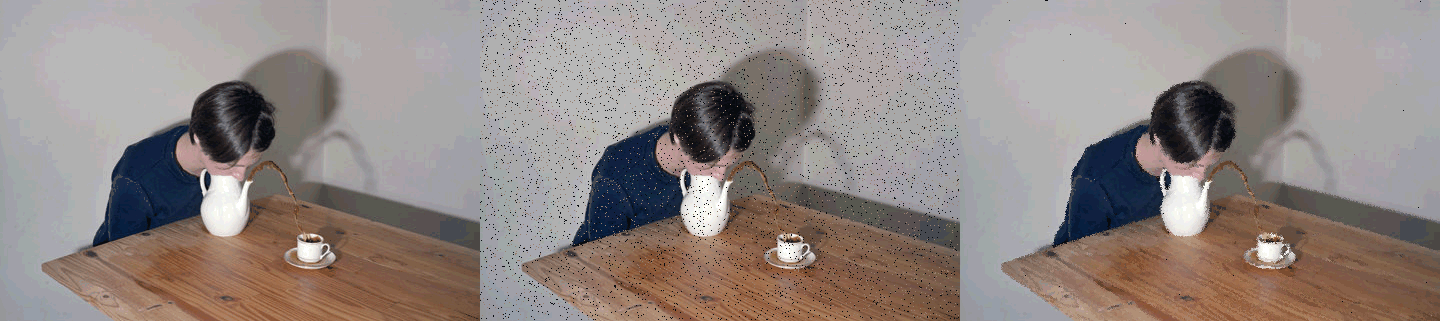
\includegraphics[width=.95\textwidth]{teapot_ensemble} %{CS0031}
\caption[Medianfilter]{Medianfilter\footnotemark}
\label{fig:Medianfilter}
\end{figure}
\footnotetext{\url{http://www.mathworks.com/help/releases/R2013b/images/ref/referencemtoz2.gif}}
\footnotetext{\url{http://bitchslapmag.com/2013/art/thomas-mailaenders-amazingly-weird-images/}}

\emph{Extremalspannenfilter}
\emph{Prewitt-Operator}
\emph{Dekonvolution}
\subsubsection{Geometrische Bilderoperationen}
Geometrische Bildoperation dienen zur Ver�nderung der Gr��e, Form und Topologie von Bildern. 

Die folgende geometrische Bildoperation verkleinert das Bild um den Faktor 2.
\begin{quote}
\textit{ErgebnisPixel( x, y ) = Ursprungsbild( x * 2, y * 2 )}
\end{quote}

\begin{figure}
\centering
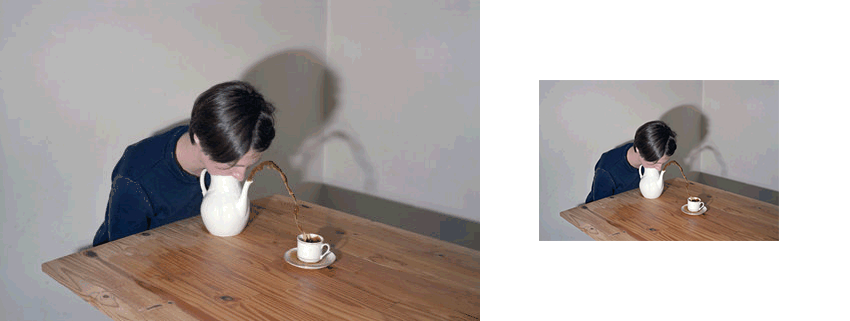
\includegraphics[width=.95\textwidth]{bildverkleinerung} %{CS0031}
\caption[Bildverkleinerung]{Bildverkleinerung}
\label{fig:Bildverkleinerung}
\end{figure}

Weiterhin kann mit geometrischen Bildoperationen unter Anderem die \emph{Skalierung}, \emph{Rotierung} oder \emph{Translation} von Bildern erreicht werden.

\subsection{Bildberarbeitung}
Bildbearbeitung bedeutet die Ver�nderung ( Verbesserung, Verfremdung oder Manipulation ) vorhandener digitaler Bilder mit ensprechender Software, wie zum Beispiel Adobe Photoshop\footnote{\url{http://www.adobe.com/}}. Diese Ver�nderung geschieht mit dem Anreiz den Eindruck des Bildes auf das menschliche Auge zu ver�ndern. Dort liegt der entscheidende Unterschied zu Bildverarbeitung, welche im vorangehenden Punkt beschrieben wurde. Es werden f�r die Bildbearbeitung zwar Algorithmen die der Bildverarbeitung zuzuordnen sind genutzt, allerdings ist der 'Konsument' des Bildes bei der Bildbearbeitung das menschliche Auge und bei der Bildverarbeitung die Maschine, bzw. weitere Algorithmen, die auf Pixelebene arbeiten.

\subsubsection{Weichzeichnen}
\subsubsection{Farbstichanpassungen}
\subsubsection{Zurechtschneiden}

\subsection{Maschinelles Sehen} 
%http://de.wikipedia.org/wiki/Maschinelles_Sehen 
Das Maschinelle Sehen erzeugt anhand eines Bildes / Bildsignales Interpretationen bzw. Bildbeschreibung des Bildes.

\subsection{Computer Vision}

\subsection{Computergrafik} 
Die Computergrafik besch�ftigt sich damit anhand von Bildbeschreibungen Bilder zu erzeugen.

\subsection{Bildvorverarbeitung} 
W�hrend der Bildvorverarbeitung k�nnen unterschiedliche Bildverarbeitungsalgorithmen auf ein Bild angewendet werden. 


\subsection{Segmentierung}
%http://de.wikipedia.org/wiki/Segmentierung_(Bildverarbeitung) 
Die Segmentierung ist ein Teilgebiet der digitalen Bildverarbeitung und des maschinellen Sehens.

Die Segmentierung ist ein Schritt/Prozess der Bildverarbeitung, in dem Regionen eines Bildes als inhaltlich zusammenh�ngend erkl�rt werden. Typischerweise geht der Segmentierung eine Vorverarbeitung voraus und folgt eine Merkmalsextraktion anhan

\section{Konkret}
\subsection{Vorverarbeitung}
\subsubsection{background subtraction}
\subsubsection{smoothing}
\subsubsection{median filter}
\subsubsection{erosion / dilatation}
\subsubsection{pyrDown / pyrUp}
\subsection{Bewegungserkennung}
\subsubsection{Optical Flow Farneback sparse/dense}
\subsubsection{Optical flow Lukas kanade sparse/dense}
\subsubsection{Opticval Flow Block Matching dense}
\subsubsection{Optical Flow Brox dense}
\subsubsection{Optiucal Flow DualTVL1}
\subsubsection{Optical Flow Horn Schunk}
\subsection{Objekterkennung}
\subsubsection{blob detection}
\subsection{Objektverfolgung}
\subsubsection{Kalman filter}
\chapter{Definition}
\section{OpenCV}
\subsection{Installation}
Da die Geschwindigkeit des Programmes von Anfang an wichtig ist wurde sich dazu entschieden so viel arbeitslast wie m�glich zu parallelisieren. Die Parallelsierung von Bildverarbeitsungsaufgaben bietet sich regelrecht an, da die Algorithmen wie folgt arbeiten: sie wenden die gleiche berechnung auf sehr viele zahlen/pixel an. Diese Arbeitsweise der Algorithmen �hnelt sehr stark der Arbeitsweise der GPU jeder Grafikkarte. 
Deswegen wurde sich dazu entschieden so viel wie m�glich der Arbeitslast auf die GPU auzulagern, da zu beginn der Bearbeitung vermutet wurde, dass eine Sequenzielle bearbeitung der Berechnungen nicht ausreichen wird, da die Software in Echzeit Videodaten verarbeiten k�nnen soll.
OpenCV unterst�tzt seit der version 2.4.6. die benutzung der CUDA Runtime API und unterst�tzt ausschlie�lich NVIDIA GPU's. Um die GPU f�r OpenCV zu benutzen muss OpenCV eigenst�ndig gebaut werden, die vorkompilierten versionen sind ohne CUDA support kompiliert. Daf�r muss CUDA , die neuesten Grafikkartentreiber und eine NVIDIA Grafikkarte vorhanden sein. 
Die Kompilierung hat sich als etwas kompliziert herausgestellt, sodass die neueste version von \url{http://www.github.com/itseez/opencv}  mit dem tag 2.4.7. benutzt werden musste um eine erfolgreiche kompilierung abzuschlie�en. Daf�r ist die Option WITH\_CUDA zu aktivieren, worauf man zus�tzlich das Verzeichnis der NVIDIA CUDA installation angeben muss. Weiterhin habe ich OpenGL f�r die beschleunigte videodarstellung und OpenMP f�r die parallelisierung auf den CPUs aktiviert, um die die Grundbedingungen f�r die Geschwindigkeit der Software ausreichend zu erf�llen.
\subsection{Mat}
In OpenCV werden s�mtliche Bilddaten als Matrizen abgebildet und der entsprechende Datentyp zur programmatischen Speicherung von Bilddaten heisst ensprechend Mat. Dieser Datentyp h�lt einige Informationen, wie die Gr��e des Bildes und der \emph{Typ} des Bildes. Die Gr��e beschreibt schlichtweg, wieviele Bildpunkte das Bild in der horizontalen, sowie in der vertikalen besitzt. Der Typ beschreibt, was f�r Bilddaten gespeichert sind. Wie bereits im Kapitel (??GRUNDLAGEN??) beschrieben k�nnen Bilder in unterschiedlichen Formaten, wie z.B. Grauwerte und Farbwerte gespeichert werden. OpenCV geht dar�ber hinaus und erm�glicht dem Entwickler zu bestimmen, wieviele \emph{channels} ein Bild hat und wie genau die Farbwerte gespeichert sind: \emph{depth}. Der Tabelle types k�nnen die diversen unterschiedlichen Typen entnommen werden.
\begin{table}
\caption[Mat Typen in OpenCV]{Mat Typen in OpenCV\footnotemark}
\label{tab:types}
\centering
\setlength{\tabcolsep}{5mm}	% separator between columns
\def\arraystretch{1.25}			% vertical stretch factor (Standard = 1.0)
\begin{tabular}{|r||c|c|c|c|} \hline
& \emph{C1} & \emph{C2} & \emph{C3} & \emph{C4}\\
\hline\hline
CV\_8U & 0 & 8 & 16 & 24\\
\hline
CV\_8S & 1 & 9 & 17 & 25\\
\hline
CV\_16U & 2 & 10 & 18 & 26\\
\hline
CV\_16S & 3 & 11 & 19 & 27\\
\hline
CV\_32S & 4 & 12 & 20 & 28\\
\hline
CV\_32F & 5 & 13 & 21 & 29\\
\hline
CV\_64F & 6 & 14 & 22 & 30\\
\hline
\end{tabular}
\end{table}
\footnotetext{\url{http://ninghang.blogspot.de/2012/11/list-of-mat-type-in-opencv.html}}

\section{Grafische Benutzeroberfl�che}
Es wird ein Framework zur gestaltung und umsetzung der grafischen Benutzeroberfl�che genutzt werden m�ssen. Die Anforderungen an dieses Framework sind eindeutig: Es muss in C++ geschrieben sein, viele g�ngige Oberfl�chenelemente anbieten und frei benutzbar sein. Im folgenden werden zwei Frameworks verglichen.
\subsection{Qt}
Qt existiert zur Zeit unter der Version 5.1.1. und ist eines der meist verbreitetsten C++ Bibliotheken zur Erstellung von grafischen Benutzeroberfl�chen. Qt's Entwicklungsgeschichte reicht bis zum Jahr 1991 zur�ck, wo die tats�chliche Entwicklung begann, allerdings wurde die erste Version im Jahr 1998 von der norwegischen Firma \textit{TrollTech} ver�ffentlicht. Qt bietet eine vielzahl von grafischen Steuerelementen, einen Qt Creator an, mit dem die Steuerelemente interaktiv angeordnet werden k�nnen und sogar ein Modul zur �bersetzung der Texte, die im Interface vorkommen in andere Sprachen, dem Linguist. Zudem wird Qt aktiv weiterentwickelt und die aktuelle Version 5.1. wurde im Juli 2013 ver�ffentlicht. Weiterhin hat Qt ein interessantes Lizensierungsmodell. Seitdem Nokia das Projekt 2008 aufkaufte wurde, wird es seit Oktober 2011 als freie Software unter der LGPL weitergegeben. Durch die LGPL ist es m�glich auch ohne eine kostenflichtige Lizenz kostenpflichtige Software mit Qt zu entwickeln, ohne den Sourcecode der Software ver�ffentlichen zu m�ssen. Ausschlie�lich, wenn �nderungen am Quellcode von Qt selbst vorgenommen wurden, m�ssen diese �nderungen ver�ffentlicht werden. 
\begin{figure}
\centering
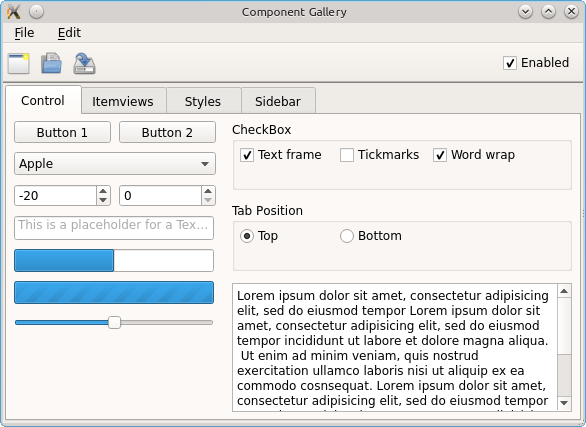
\includegraphics[width=.95\textwidth]{qt_gallery} %{CS0031}
\caption[Qt Steuerelemente]{Qt Steuerelemente\footnotemark}
\label{fig:Qt Steuerelemente}
\end{figure}
\footnotetext{\url{http://www.ics.com/blog/whats-new-qt-51-qt-quick-controls}}

\subsection{Alternativen}
In diesem Kapitel wird auf die alternativen Frameworks und Bibliotheken zum Qt-Project eingegangen.
\subsubsection{Windows Template Library}
WTL\footnote{\url{http://wtl.sourceforge.net/}} ist eine Bibliothek zur Entwicklung von grafischen Benutzeroberfl�chen f�r Windows. Sie ist unter der CPL lizensiert, besitzt ebenfalls diverse Steuerelemente, kann allerdings ausschlie�lich unter Win32 Anwendungen benutzt werden.
\begin{figure}
\centering
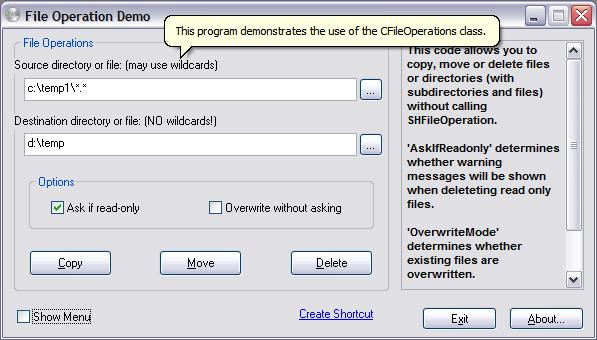
\includegraphics[width=.95\textwidth]{wtl_example} %{CS0031}
\caption[WTL Beispiel]{WTL Beispiel\footnotemark}
\label{fig:WTL Beispiel}
\end{figure}
\footnotetext{\url{http://www.codewiz51.com/wiki/GetFile.aspx?File=WTLFopDemonstration/WTLFopDemonstrationNoMenu.JPG}}
\subsubsection{wxWidgets}
wxWidgets\footnote{}\url{http://www.wxwidgets.org/} ist eine C++ Bibliothek, die die Entwicklung von grafischen, plattform�bergreifenden Anwendungen unterst�tzt.
wxWidgets ist under der "wxWidgets License" lizensiert, welche grunds�tzlich der L-GPL Lizenz entspricht, allerdings mit dem Unterschied, Software, die wxWidgets in bin�rer Form nutzt eigene Lizensierung anwenden kann\footnote{\url{http://www.wxwidgets.org/about/newlicen.htm}}.
\subsubsection{gtkmm}
gtkmm ist eine offizielle C++ Anbindung an die GTK+ Bibliothek. Sie bietet viele �bliche Oberfl�chenelemente an, und bietet die M�glichkeit diese per Vererbung noch anzupassen. Die Benutzeroberfl�che kann per Quellcode, aber auch mithilfe des \textit{Glade User Inteface Designer}s\footnote{}\url{http://glade.gnome.org/} erstellt werden.
\begin{figure}
\centering
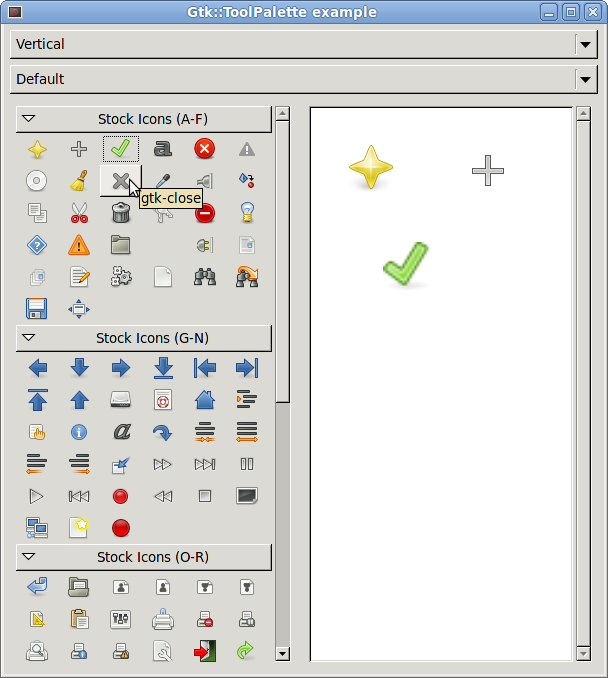
\includegraphics[width=.95\textwidth]{gtkmm_palette} %{CS0031}
\caption[gtkmm Toolpalette]{gtkmm Toolpalette\footnotemark}
\label{fig:gtkmm Toolpalette}
\end{figure}
\footnotetext{\url{https://developer.gnome.org/gtkmm-tutorial/3.4/toolpalette-example.html.en}}
Weiterhin ist gktmm unter der LGPL Lizenz ver�ffentlicht\footnote{\url{http://www.gtkmm.org/en/license.shtml}}.
\chapter{Tests}
In diesem Kapitel wird die Software getestet. Sie wird auf Grundlage der Kriterien aus dem Kapitel Anforderungsanalyse untersucht, inwiefern sie den urspr�nglichen Anspr�chen entspricht und wo sie ggf. nicht eingehalten werden konnten.

\section{Benchmarks}
In diesem Abschnitt wird auf die Geschwindigkeit der verwandten Algorithmen eingegangen. Als Referenz, die Hardware auf der die Tests durchgef�hrt wurde hatte folgende Konfiguration:
Intel i7-3720QM, einer NVidia Quadro K1000M, 8GB DDR3 RAM 1600MHz.

\section{Funktion}
\chapter{Zukunftsaussichten}
F�r die Zukunft k�nnte ein System entwickelt werden, welches Schiffe sogar ausgesprochen schnell auf kosteng�nstiger Hardware erkannt werden k�nnte. Dieser Ansatzt spaltet das gesammte System in zwei Teile. Diese beiden Teile sind jeweils voneinander abgekoppelte Applikationen, wobei die erstApplikation im gro�en und ganzen der in dieser AStbeit beschriebenen gleicht. Der entscheidende Unterschied jodoch liegt darin, dass diese Sofware nicht unmittelbar daf�r benutzt wird, Schiffe zu erkennen und zu tracken, sondern lediglich daf�r benutzt wird einen Machine-Learning Algorithmus wie z.B. den Haar-Classifier zu trainieren. Dadurch kann die Software nach kurzer vorangegangener Parameterkalibierung eigenst�ndig Bilder von Schiffen erkennen und speichern, welche darauf zum Training des Haar-Klassifiers benutzt werden.
Der zweite Teil des Systemes w�re ein Computer mit Raspberry-Pi-�hnlicher Architektur und Leistung, welcher daf�r zust�ndig ist das digitale Videosignal ausschliesslich anhand eines Haar-Klassifiers zu analysieren, was selbst auf der heutzuztage billigsten Hardware in Echtzeit m�glich ist. (30euro RaspPi)
\chapter{Quellen}
[Sester01]
\url{http://docs.opencv.org/2.4.5/modules/nonfree/doc/background_subtraction.html}
\url{http://docs.opencv.org/doc/tutorials/imgproc/gausian_median_blur_bilateral_filter/gausian_median_blur_bilateral_filter.html}
\url{http://docs.opencv.org/doc/tutorials/imgproc/pyramids/pyramids.html}
\url{http://docs.opencv.org/modules/video/doc/motion_analysis_and_object_tracking.html#segmentmotion}


\end{document}